\documentclass[aspectratio=169]{wzbeamer}
\usepackage[hyperref=true,style=numeric,backend=biber,sorting=nty,autocite=inline,backref=true,urldate=iso,date=iso,seconds=true]{biblatex}
\addbibresource{ref.bib}
\usepackage{animate}
\usetheme[progressbar=frametitle, numbering=counter]{metropolis}
\usepackage{fontspec}
\setmainfont{Times New Roman}
\setsansfont{Arial}
\setmonofont{Cambria}

\usepackage{etoolbox} % for '\AtBeginEnvironment' macro
\AtBeginEnvironment{pmatrix}{\everymath{\displaystyle}}

\graphicspath{{./figs/}}

\title{Liouville's Theorem and Jarzynski Equality}
\subtitle{平统讨论班}
\author{王准}
\institute[pku]{北京大学}


\begin{document}
\maketitle 
    
\begin{frame}{Overview}
    \tableofcontents
\end{frame}


\section{Liouville定理}
    \subsection{定理证明}
    \begin{frame}{Liouville定理}
        \begin{alertblock}{Liouville定理}
            系统按照满足哈密顿正则方程演化时, 微观态密度分布沿系统轨迹保持为常数, 即,
            \begin{equation}
                \dv{\rho}{t} = 0
            \end{equation}
        \end{alertblock}

    \end{frame}
    \begin{frame}{证明1}
        哈密顿量$H = H(\vb*q, \vb*p) = H(\vb*x)$, $\vb*x = (\vb*q, \vb*p)$
        \begin{equation}
            \left\{
            \begin{split}
                \dot{q}_i &= \pdv{H}{p_i}\\
                \dot{p}_i &= - \pdv{H}{q_i}
            \end{split}
            \right.\quad
            \Rightarrow\quad
            \dot{x}_\alpha = \omega_{\alpha\beta} \pdv{H}{x_\beta}
        \end{equation}
        其中, $i = 1,2,\dots,n, \ \alpha = 1,2,\dots,2n$, 
        \begin{equation}
            [\omega_{\alpha\beta}] = 
            \begin{pmatrix}
                & I \\
                -I & 
            \end{pmatrix}
            \quad\Rightarrow\quad
            \omega_{\alpha\beta} = -\omega_{\beta\alpha}
        \end{equation}
    \end{frame}
    
    \begin{frame}{证明1}
        相空间中, 微观态的数量应该保持不变, 可以写出流和密度满足的守恒关系,
        \begin{equation}
            \pdv{\rho(\vb*x, t)}{t} + \pdv{x_\alpha}(\dot x_\alpha \rho(\vb*x,t) ) = 0
        \end{equation}
        从而,
        \begin{equation}
            \begin{split}
                \dv{\rho(\vb*x(t),t)}{t} =& \pdv{\rho}{t} + \dot x_\alpha \pdv{\rho}{x_\alpha}\\
                =& - \rho\cdot \pdv{x_\alpha}\dot x_\alpha\\
                =& - \rho\cdot \omega_{\alpha\beta} \pdv{H}{x_\alpha}{x_\beta}\\
                =& \ 0
            \end{split}
        \end{equation}
    \end{frame}
    \begin{frame}{证明2}
        从演化的角度考虑, 微观态数目不变可以表述为,
        \begin{equation}
            \rho(\vb*x_t,t) \dd\vb*x_t = \rho(\vb*x_0,0) \dd\vb*x_0, \quad\vb*x_t = \vb*x(t)
        \end{equation}
        其中, $\dd\vb*x_t$表示体积元. 我们如果将时间演化视作一种变换, 
        \begin{equation}
            \phi_{s\to t} : \vb*x_s \mapsto \vb*x_t,\quad \text{i.e.}\ \vb*x_t = \phi_{s\to t} (\vb*x_s)
        \end{equation}
        那体积元之间的关系就应该由Jacobi行列式决定,
        \begin{equation}
            \dd\vb*x_t = \det(\pdv{\vb*x_t}{\vb*x_0}) \dd\vb*x_0 = J(t) \dd\vb*x_0
        \end{equation}
    \end{frame}
    \begin{frame}{证明2}
        求$J(t)$对时间的导数,
        \begin{equation}
            \begin{split}
                \dv{J}{t} &= \sum_\alpha \det(\pdv{(\dots ,\dot x_{t, \alpha}, \dots)}{\vb*x_0})\\
                &= \sum_\alpha \det(\pdv{(\dots ,\dot x_{t,\alpha}, \dots)}{\vb*x_t}) \cdot J(t)\\
                &= \sum_\alpha \pdv{\dot x_{t, \alpha}}{x_{t,\alpha}}\cdot J\\
                &= \omega_{\alpha\beta} \pdv{H}{x_{t,\alpha}}{x_{t,\beta}}\cdot J\\
                &= \ 0
            \end{split}
        \end{equation}
        $$ J \equiv 1 \quad \Rightarrow\quad \rho(\vb*x_t, t) = \rho(\vb*x_0, 0)$$ 
    \end{frame}
    \begin{frame}{Jacobi矩阵}
        Jacobi矩阵实际上就是向量函数对于向量自变量的导数, 
        \begin{equation}
            \pdv{\vb*y}{\vb*x} = [\pdv{y_i}{x_j}] = 
            \begin{pmatrix}
                \pdv{y_1}{x_1} & \pdv{y_1}{x_2} & \cdots & \pdv{y_1}{x_n}\\
                \pdv{y_2}{x_1} & \pdv{y_2}{x_2} & \cdots & \pdv{y_2}{x_n}\\
                \vdots & \vdots & & \vdots\\
                \pdv{y_n}{x_1} & \pdv{y_n}{x_2} & \cdots & \pdv{y_n}{x_n}
            \end{pmatrix}
        \end{equation}
        求导的链式法则也可以扩展到这个情形,
        \begin{equation}
            \pdv{\vb*z}{\vb*x} = \pdv{\vb*z}{\vb*y} \cdot \pdv{\vb*y}{\vb*x}
        \end{equation}
    \end{frame}
    \begin{frame}{证明2}
        证明2实际上给了一种新的观点, $\phi$是一个保持体积元大小不变的映射, 那么$\phi$就应该保持体积不变. 设$m$是相空间的Lebesgue测度(实际上就是体积), 对于可测集$A$,
        \begin{gather}
            m(A) = \int_A \dd \vb*x\\
            m(\phi(A)) = m(A)
        \end{gather}
        利用这一点, 我们可以将Poincar\'e定理运用到时间演化上.
    \end{frame}
    \subsection{Poincar\'e定理}
    \begin{frame}{Poincar\'e定理}
        \begin{alertblock}{Poincar\'e定理(数学表述)}
            对于有限测度空间$(X,\Sigma,\mu)$, 若$f$是一个保测度的映射, 那么, $\forall E\in\Sigma$, 
            \begin{equation}
                \mu(\{x\in E: \exists N, \forall n > N, f^{\ n}(x) \notin E \}) = 0
            \end{equation} 
            即, 几乎所有的点都会在有限步回到$E$中.
        \end{alertblock}
    \end{frame}
    \begin{frame}{证明思路}
        令 $A_n = \bigcup_{k=n}^{\infty} f^{-k}E$, 表示了$E$中的点在$n$步以前的位置, 显然$E\subset A_0,\ \mu(A_n) = \mu(A_m)$, 
        \begin{equation}
            \mu(E - A_n) \leqslant \mu(A_0 - A_n) = \mu(A_0) - \mu(A_n) = 0
        \end{equation}
        而$\mu(E - \bigcap_{n=1}^\infty A_n) = \mu(\bigcup_{n=1}^\infty (E - A_n)) = 0 $, 表示了在所有在有限步没有回到$E$中的点.
    \end{frame}
    \begin{frame}{微正则系综中构造有限测度}
        微正则系综处于一个能壳$E\sim E+\dd E$上, 取$\dd n$为法向的线元, 我们有
        \begin{equation}
            |\nabla E|\dd n = \dd E  
        \end{equation}
        而我们知道时间演化是保持体积元的, 即$\dd S\dd n == \dfrac{\dd S}{|\nabla E|} \dd E$在时间演化下不变, 那么构造测度$\mu$,
        \begin{equation}
            \mu(A) = \int_A \frac{\dd S}{|\nabla E|}
        \end{equation}
        由于能壳总面积有限, 这是一个有限测度, 所以可以应用Poincar\'e定理. 即, 一个集合内的态几乎总会在有限时间的演化后回到初始的集合内.
    \end{frame}
    \begin{frame}{Poincar\'e定理和各态历经}
        统计物理中一个很重要的假设是各态历经, 它和Poincar\'e定理非常相似.
        \begin{itemize}
            \item 各态历经, 任意一个非零测度的集合$E$, 全空间$X$中最终不会到达$E$的点的测度为零.
            \item Poincar\'e, 任意一个非零测度的集合$E$, 从$E$出发最终不会到达$E$的点的测度为零.
        \end{itemize}
    \end{frame}
    
\section{Jarzynski等式}
    \subsection{发展过程}
    \subsection{等式证明}
    \begin{frame}{Jarzynski等式}
        \begin{columns}
            \column{.7\textwidth}
            \begin{alertblock}{Jarzynski等式}
                对于一个和大热库(温度为$T$)有热交换的系统, 从一个平衡态$A$出发, 由外界改变系统的某些宏观参数, 从而使得系统经历一个演化过程, 最后到达一个新的平衡态$B$, 对于系统的自由能$F$, 和过程中的做功$W$满足,
                \begin{equation}
                    \exp (- \frac{\Delta F}{k_B T}) = \expval{\exp (- \frac{W}{k_B T})},\quad \Delta F = F_B - F_A
                \end{equation}
                其中, $\expval{\cdot}$表示对于初始状态$A$的正则系综取平均.
            \end{alertblock}
            \column{.3\textwidth}
            \begin{figure}[H]
                \centering
                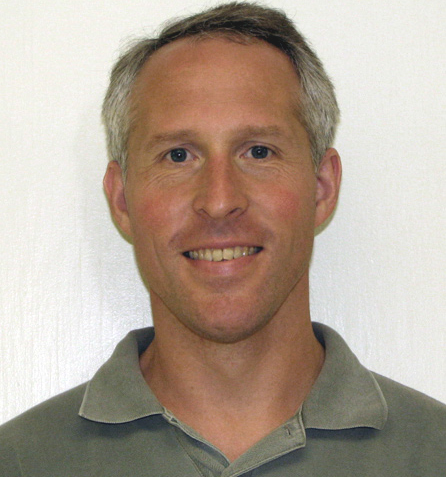
\includegraphics[width=.9\textwidth]{jarz.jpg}
                \caption{Christopher Jarzynski}
            \end{figure}
        \end{columns}
    \end{frame}
    \begin{frame}{详细解释}
        \begin{columns}
            \column{.6\textwidth}
            \begin{itemize}
                \item 外界改变宏观参数, 但演化仍然满足正则方程, $H_\lambda(\vb*q,\vb*p)$
                \item 参数改变的路径是确定的, 关于时间的函数关系不受限制, $\gamma$
                \item 过程中可以是非平衡态, 但是初末态是平衡态, 且温度相同
            \end{itemize}
            \column{.4\textwidth}
            \begin{figure}[H
                ]
                \centering
                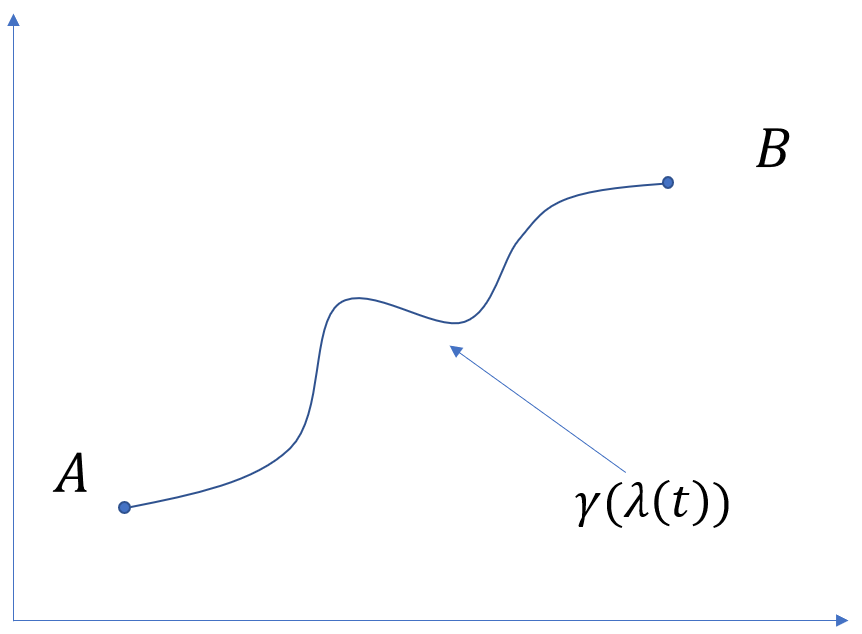
\includegraphics[width=\textwidth]{parameter.png}
                \caption{参数空间变化}
            \end{figure}
        \end{columns}
    \end{frame}
    \begin{frame}{证明}
        我们先考虑孤立系统的情况, 假设曲线参数$\lambda\in[0,1]$, 哈密顿量为$H_\lambda(\vb*x)$, 外界对系统做功,
        \begin{equation}
            W = \int_0^{t_s} \dd t \dot\lambda \pdv{H_\lambda(\vb*x(t))}{\lambda}
        \end{equation}
        极限情形, $\dot\lambda \to \infty, t_s\to 0$, 这样系统参数瞬时变化, 
        \begin{gather*}
            W = \int_0^1 \dd\lambda\pdv{H_\lambda(\vb*x(0))}{\lambda} = H_1(\vb*x(0)) - H_0(\vb*x(0)) \\
            \expval{\ee^{-\beta W}} = \int_\Gamma\dd\vb*x_0 \dfrac{\ee^{-\beta H_0(\vb*x_0)}}{Z_0} \cdot \ee^{-\beta (H_1(\vb*x_0) - H_0(\vb*x_0))} = \frac{Z_1}{Z_0}
        \end{gather*}
    \end{frame}
    \begin{frame}{证明\ --\ 极限情形}
        极限情形, $\dot\lambda \to \infty, t_s\to 0$, 这样系统参数瞬时变化, 
        \begin{gather*}
            W = \int_0^1 \dd\lambda\pdv{H_\lambda(\vb*x(0))}{\lambda} = H_1(\vb*x(0)) - H_0(\vb*x(0)) \\
            \expval{\ee^{-\beta W}} = \int_\Gamma\dd\vb*x_0 \dfrac{\ee^{-\beta H_0(\vb*x_0)}}{Z_0} \cdot \ee^{-\beta (H_1(\vb*x_0) - H_0(\vb*x_0))} = \frac{Z_1}{Z_0}
        \end{gather*}
        而若$\dot\lambda \to 0$, 系统准静态演化, 可逆过程所有的做功都等于$\Delta F$, 
        $$
        \expval{\ee^{-\beta \Delta F}} = \ee^{-\beta \Delta F}
        $$
    \end{frame}
    \begin{frame}{证明\ --\ 一般情形}
        变积分变量为$\lambda$, 那么应当有$t = t(\lambda), \vb*x(t) = \vb*x(t(\lambda))$
        \begin{equation}
            \begin{split}
                \dv{H_\lambda(\vb*x(t(\lambda)))}{\lambda} &= \pdv{H_\lambda}{\lambda} + \pdv{H_\lambda}{x_\alpha} \dot x_\alpha\cdot \frac1{\dot\lambda}\\
                &= \pdv{H_\lambda}{\lambda} + \omega_{\alpha\beta}\pdv{H_\lambda}{x_\alpha}\pdv{H_\lambda}{x_\beta}\\ 
                &= \pdv{H_\lambda}{\lambda}
            \end{split}
        \end{equation}
        因此,
        \begin{equation}
            W = \int_0^1 \dd \lambda \dv{H_\lambda}{\lambda} = H_1(\vb*x(t_s)) - H_0(\vb*x(0))
        \end{equation}
    \end{frame}
    \begin{frame}{证明}
        再经过一段时间的弛豫, 到达平衡态, 此过程外界不做功, 微观自由度按照正则方程演化
        $$H_1(\vb*x(t_f)) = H_1(\vb*x(t_s))$$
        因此,
        \begin{equation}
            \begin{split}
                \expval{\ee^{-\beta W}} &= \int_\Gamma\dd\vb*x_0 \dfrac{\ee^{-\beta H_0(\vb*x_0)}}{Z_0} \cdot \ee^{-\beta (H_1(\vb*x_{t_f}) - H_0(\vb*x_0))}\\
                &= \int_\Gamma\dd\vb*x_0 \dfrac{\ee^{-\beta H_1(\vb*x_{t_f})}}{Z_0}
            \end{split}
        \end{equation}
        由Liouville定理, $\dd\vb*x_t = \dd\vb*x_0$,
        \begin{equation}
            \expval{\ee^{-\beta W}} = \frac1{Z_0} \int_\Gamma \dd\vb*x\ \ee^{-\beta H_1(\vb*x)} = \frac{Z_1}{Z_0}
        \end{equation}
    \end{frame}
    \begin{frame}{证明}
        接下来, 我们来考虑有热库的情形, 整个系统的哈密顿量,
        \begin{equation}
            \mathscr{H}_\lambda(\vb*x,\vb*x') = H_\lambda(\vb*x) + H'(\vb*x') + h_{int} (\vb*x, \vb*x')
        \end{equation}
        把整个系统视作整体, 那么,
        \begin{equation}
            W = \mathscr H_1(\vb*y(t_f)) - \mathscr H_0(\vb*y(0)),\quad \vb*y = (\vb*x, \vb*x')
        \end{equation}
        按照孤立系统的结论,
        \begin{equation}
            \int_{\Gamma\times\Gamma'}\dd\vb*y_0 \frac{\ee^{-\beta\mathscr H_0}}{\mathscr Z_0} \cdot \ee^{-\beta W} = \frac{\mathscr Z_1}{\mathscr Z_0}
        \end{equation}
    \end{frame}
    \begin{frame}{证明\ -- \ 对于相互作用项的近似}
        
    \end{frame}
    % \begin{frame}{gif page}
    %     \begin{figure}[H]
    %         \centering
    %         \animategraphics[width=.8\textwidth]{10}{gif/anim}{0}{39}
    %         \caption{变化}
    %     \end{figure}
    % \end{frame}
    \subsection{实验}

\section{涨落定理}
    \subsection{Crooks Fluctuation Theorem(CFT)}
    \subsection{Transient Fluctuation Theorem(TFT)}


%====================================================================================
% \begin{frame}[allowframebreaks]
%     \nocite{*}
% 	\frametitle{References}
% 	\printbibliography[title={References}]
% \end{frame}
\end{document}